\subsection{Overview}

This section provides a high-level overview of the system architecture, detailing its main components and the interactions among architectural layers. It also describes the modeling decisions made to satisfy both the functional and non-functional requirements defined in the RASD document.

\subsubsection{System View}

The BBP system adopts a microservices-based architecture ~\cite{microservices_pattern} to support the scalable and independent evolution of user management, trip tracking, and bike-path management functionalities. The architecture is organized into several tiers. 
\begin{enumerate}
    \item \textbf{The mobile application tier} acts as the presentation layer, providing all user interfaces.
    \item \textbf{The API gateway tier} receives client requests and routes them to the appropriate microservices.
    \item \textbf{The microservices tier} contains the set of services that implement BBP’s core business capabilities.
    \item \textbf{The data tier} ensures that each service owns and accesses its dedicated storage.
    \item \textbf{The external services tier} represents the external APIs and systems consumed by BBP.
\end{enumerate}

This architectural style improves fault isolation and allows each service to be deployed, scaled, and maintained independently as usage patterns evolve, for example when trip recording or path search become more demanding than user registration.

\begin{figure}[H]
\centering
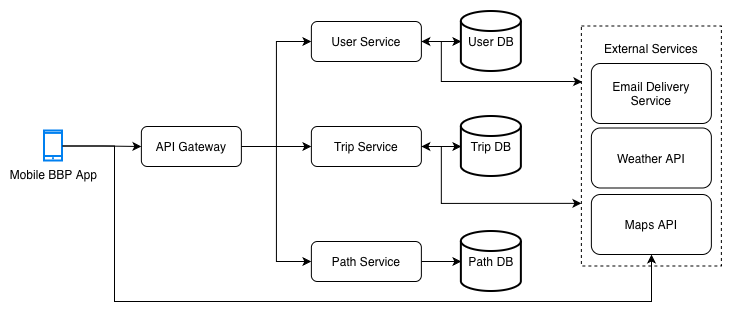
\includegraphics[width=\textwidth]{DD/Images/Architecures/Architectures-High Level.png}
\caption{\label{fig:architectureDiagram}High level architecture.}
\end{figure}

\subsubsection{Detailed View}

\subsubsection*{Mobile application tier}

The Mobile BBP App is the primary client used by cyclists to register, record, and browse trips and bike paths while riding. It interacts with the backend over HTTPS, sending GPS, sensor data, and user inputs (manual path insertion, confirmation of potholes) required by the BBP domain. This client keeps only presentation and local cache, delegating computation such as statistics, scoring, and path merging to backend services to preserve consistency.

\subsubsection*{API gateway tier}

The API Gateway acts as the single entry point to the microservices landscape. It routes incoming calls to the appropriate service (User, Trip, or Path), performs authorization, applies rate limiting, and can aggregate responses so that the mobile application does not need to orchestrate multiple calls for a single screen. 

The gateway integrates a built‑in API authorizer, which validates client credentials and access tokens, evaluates access policies, and enforces fine-grained permissions before forwarding a request to any backend service. This ensures that only authenticated and authorized users can invoke protected operations, while keeping security logic centralized and consistent across the system. 

The API Gateway abstraction also hides internal service URLs, protocols, and versioning, which simplifies the mobile client and allows services to evolve, be replaced, or be scaled independently without breaking existing applications.


\subsubsection*{Microservices tier}

This tier host all the business logic of the application, separated by services. The User Service manages registration, authentication, and user profiles, supporting all features that require identifying the user. The Trip Service handles the creation, storage, and analysis of trip data. It also enriches trips with weather information retrieved from the external Weather API when available. The Path Service manages bike‑path entities, their status, and obstacle reports, and is responsible for merging publishable information from multiple users over time to derive consolidated path scores used for route visualization.

Adopting a microservices architectural style provides several advantages. Each service encapsulates a clearly defined set of responsibilities and owns its data, which reduces coupling and enables independent development, deployment, and scaling. For example, the Trip Service can be scaled horizontally to handle high‑volume sensor data without affecting the User or Path Services. Fault isolation is also improved, since a failure or performance degradation in one service (such as the integration with the Weather API) does not necessarily compromise the availability of the others. Furthermore, this decomposition allows teams to evolve the technology stack or data models of a single service with minimal impact on the rest of the system.

The architecture is designed with observability in mind. Each microservice exposes metrics, logs, and traces that can be collected and correlated by centralized monitoring and logging tools. Structured application logs, domain‑specific metrics (e.g., number of trips processed, average trip enrichment latency), and distributed tracing across User, Trip, and Path Service calls enable effective end‑to‑end monitoring of user workflows. This observability layer facilitates proactive detection of anomalies, faster diagnosis of incidents, and data‑driven capacity planning, thereby improving the reliability and maintainability of the BBP platform over time.

\subsubsection*{Data tier and External services tier}

Each microservice owns a dedicated database: User DB, Trip DB, and Path DB. Ensuring loose coupling and independent scaling of storage according to access patterns (for instance, high‑write trip data versus relatively stable user records). This database‑per‑service pattern also supports autonomy in schema evolution and technology choice, which is valuable as BBP analytics or geospatial needs grow. 

Also, dedicated integrations with the Email Delivery Service and Weather API allow services to send notifications and enrich trips with meteorological information without exposing external APIs directly to the mobile client. Isolating these integrations inside backend services keeps credentials and error handling on the server side, and shields users from third‑party outages through backend‑level resilience strategies.

\begin{figure}[H]
\centering
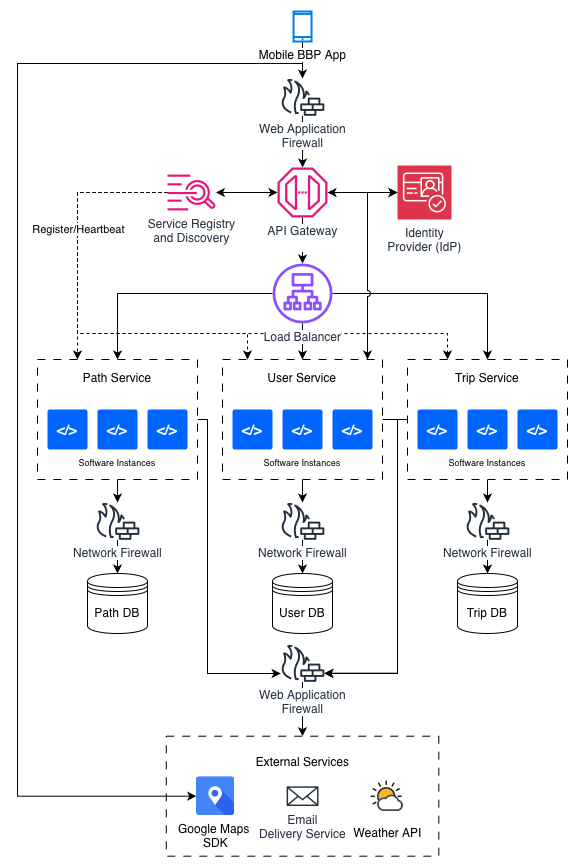
\includegraphics[width=\textwidth]{DD/Images/Architecures/Architectures-Detail.png}
\caption{\label{fig:architectureDiagram}Detailed architecture.}
\end{figure}

\subsection{Component View}

\begin{figure}[H]
\centering
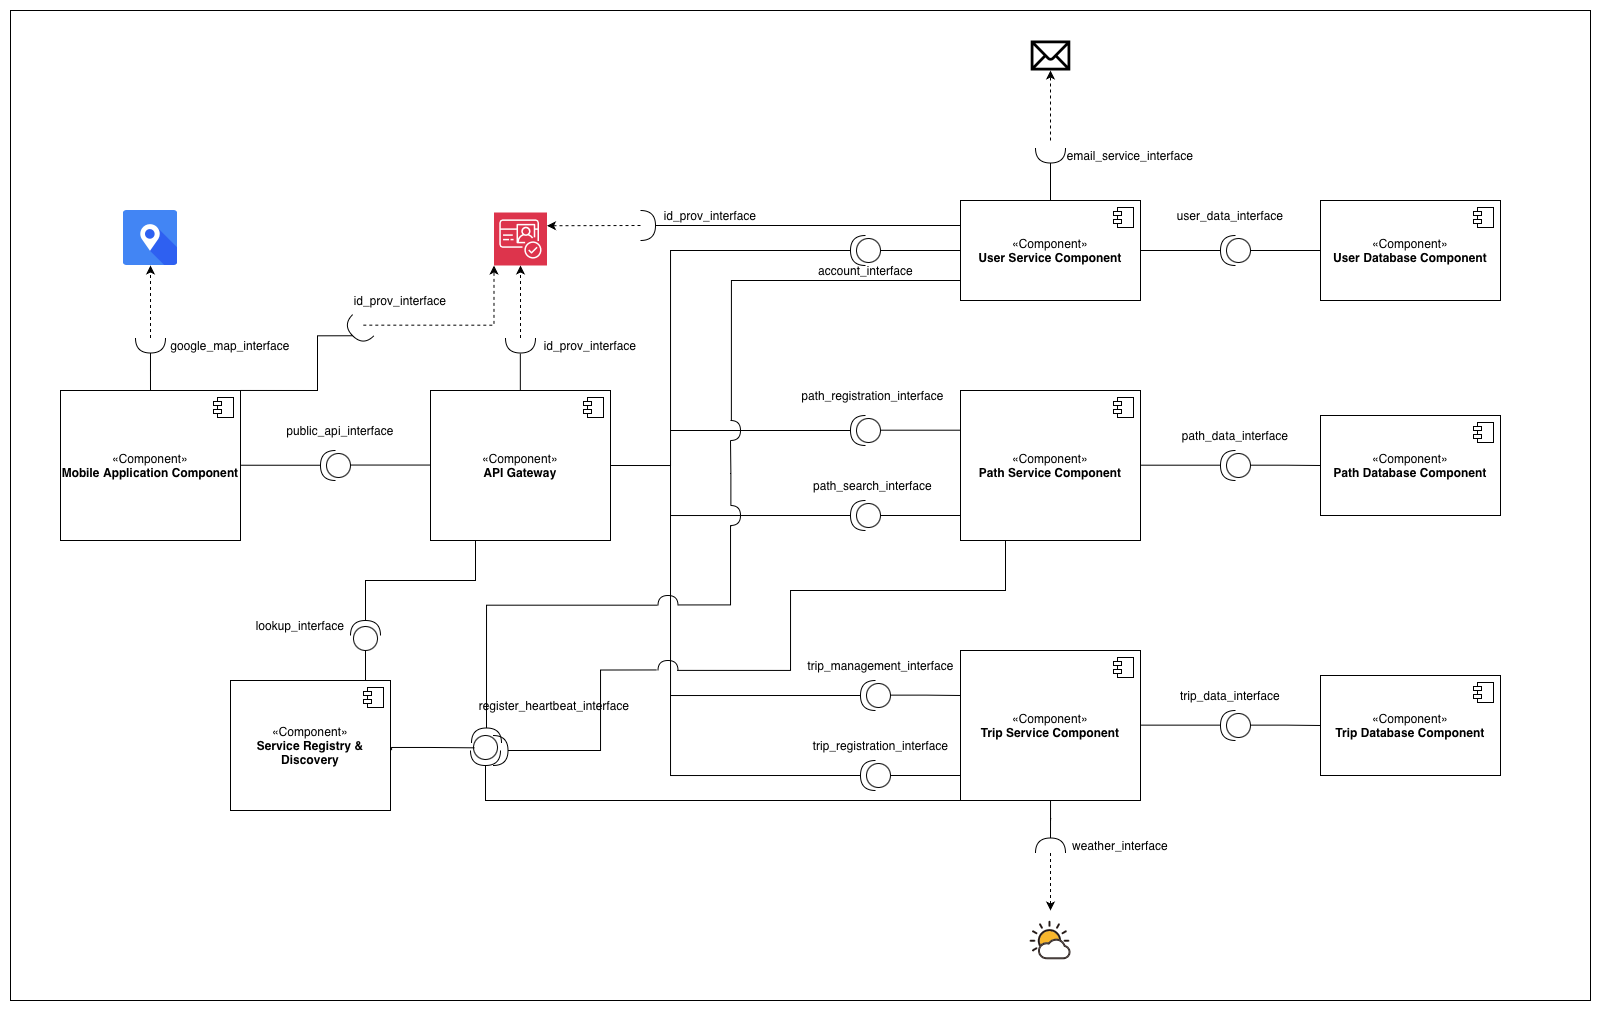
\includegraphics[width=\textwidth]{DD/Images/Component Diagrams/Component Diagram.png}
\caption{\label{fig:componentDiagram}Component Diagram.}
\end{figure}

This diagram provides a high‑level representation of the main components of the BBP system, where the application layer is modeled through the API Gateway and microservice components, while their internal structure is detailed in subsequent sections. 

The interfaces depicted on the left correspond to the interactions between the Mobile Application Component and the backend entry point, and capture the principal functionalities requested by clients, such as user management, trip registration, and path search. 

On the right side, the diagram highlights the external interfaces consumed by the backend, including the Email Delivery Service and Weather API, as well as the dedicated database components that expose data‑access interfaces for user, path, and trip information, all managed by the respective service components to satisfy the system’s persistence and integration needs.

Details regarding the microservices components are presented on figure 4 alongside the respective description.
    
\begin{figure}[H]
\centering
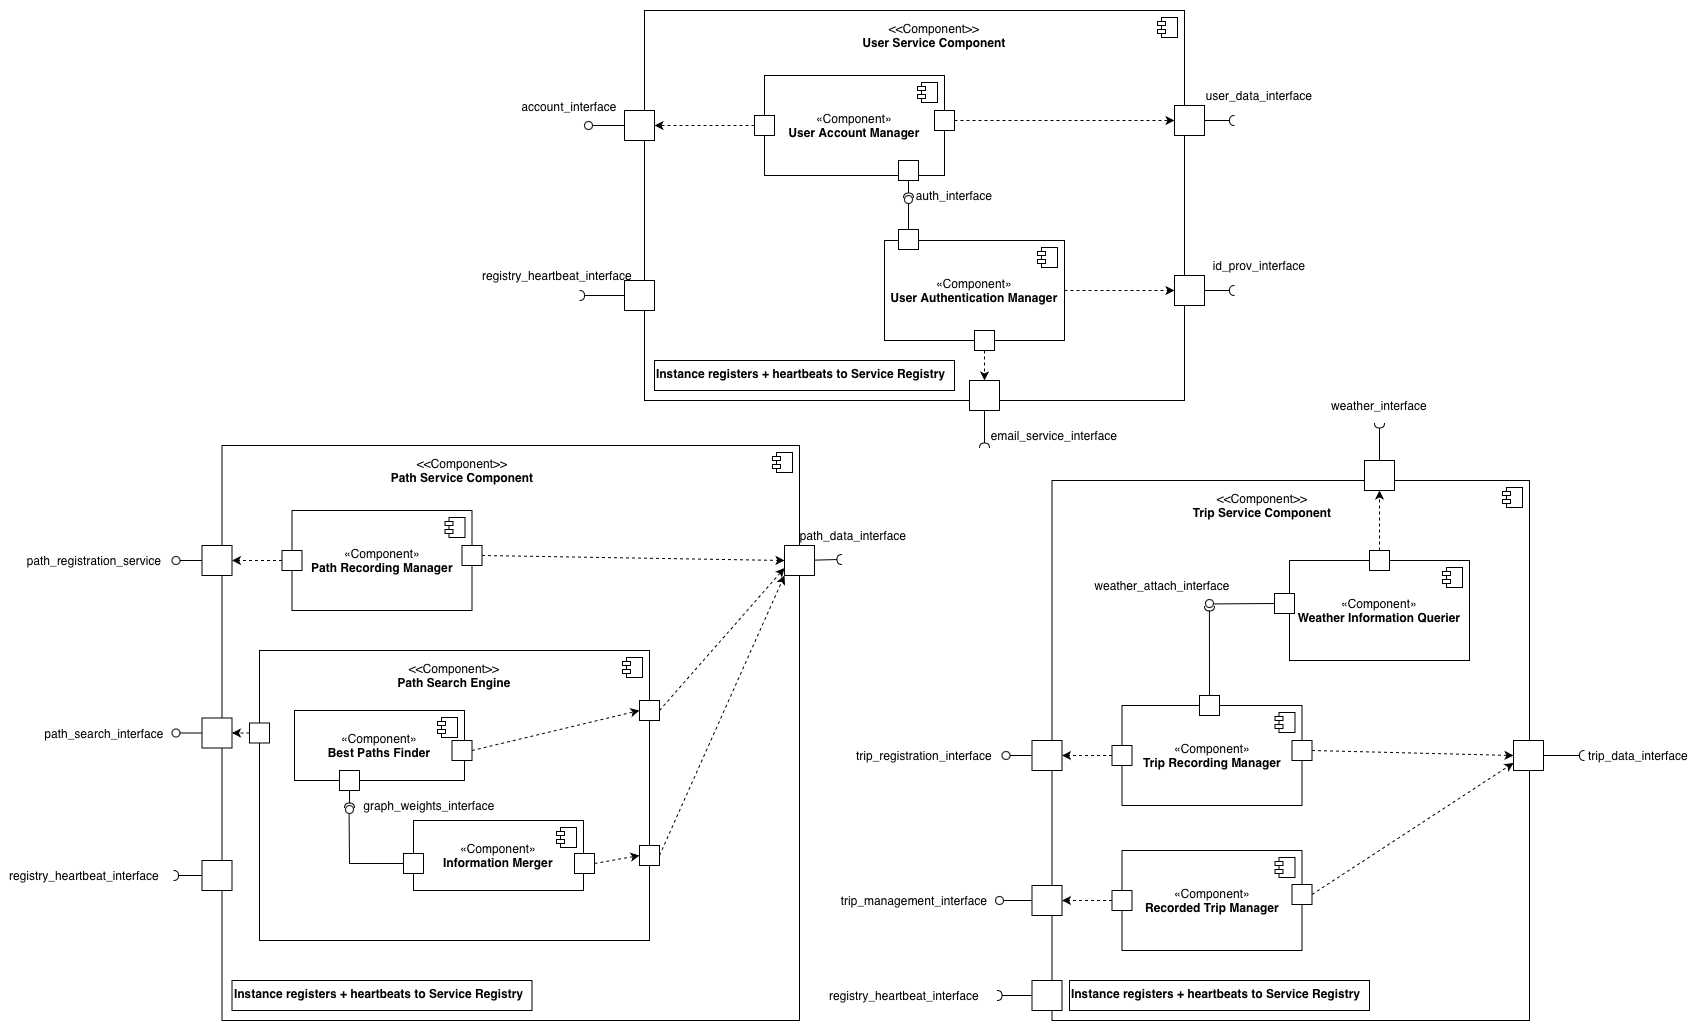
\includegraphics[width=\textwidth]{DD/Images/Component Diagrams/Detailed-Component-View.png}
\caption{\label{fig:componentDiagram} Detailed Services Component Diagram.}
\end{figure}


\subsubsection*{User Service Component}

\begin{itemize}
    \item \textbf{User Account Manager} handles core life-cycle operations for user accounts, including sign-up (user registration), login, account activation/deactivation, and deletion. This sub-component enforces business rules for account state transitions.
    \item \textbf{User Authentication Manager} manages secure access control, supporting operations such as sign-up validation, login token issuance, account confirmation, password reset flows, and sign-out. It delegates identity verification to the external Identity Provider and integrates with the Email Delivery Service for confirmation emails.
\end{itemize}

\subsubsection*{Trip Service Component}

\begin{itemize}
    \item \textbf{Weather Information Querier} retrieves meteorological data for recorded trips by invoking the external Weather API with trip timestamps and geolocations. This sub-component implements resilience patterns (timeouts, retries) and caches recent weather data to minimize external dependencies and support offline trip enrichment.
    \item \textbf{Trip Recording Manager} orchestrates the creation of new trips from mobile GPS/sensor data, invoking \texttt{CreateTrip} to persist raw trip information and scheduling \texttt{CreateWeatherJob} to asynchronously fetch and associate weather data via the Weather Information Querier.
    \item \textbf{Recorded Trip Manager} provides query interfaces for trip retrieval, supporting \texttt{GetTrips} (list user's trips with filtering/sorting) and \texttt{GetTrip} (retrieve detailed metrics like distance, average speed, and weather for a specific trip ID).
\end{itemize}

\subsubsection*{Path Service Component}

\begin{itemize}
    \item \textbf{Path Recording Manager} manages the lifecycle of bike path entities, implementing \texttt{CreatePath} (manual/automated path registration), \texttt{VerifyPath} (user confirmation/correction of detected obstacles like potholes), and \texttt{PublishPath} (promotion of verified paths to community-visible status).
    \item \textbf{Path Search Engine} computes optimal bike routes between origin/destination points by coordinating path discovery and scoring.
    \begin{itemize}
        \item \textbf{Best Paths Finder} implements \texttt{ComputePossiblePaths}, evaluating candidate routes based on path scores, distance effectiveness, and user preferences while integrating geospatial queries via Maps SDK.
        
        \item \textbf{Information Merger} aggregates publishable path data from multiple users, applying freshness weighting and confirmation counts to resolve conflicts (e.g., prioritizing ``optimal'' status from multiple recent reports over older ``requires maintenance'' tags).
    \end{itemize}
\end{itemize}


\subsection{Deployment View}

The deployment diagram shows BBP components distributed across client devices (Mobile App), security nodes (WAF, API Gateway), container hosts (microservices with load balancers), databases (Path/User/Trip DBs), and external providers (Google Maps, Email, Weather API).

\begin{figure}[H]
\centering
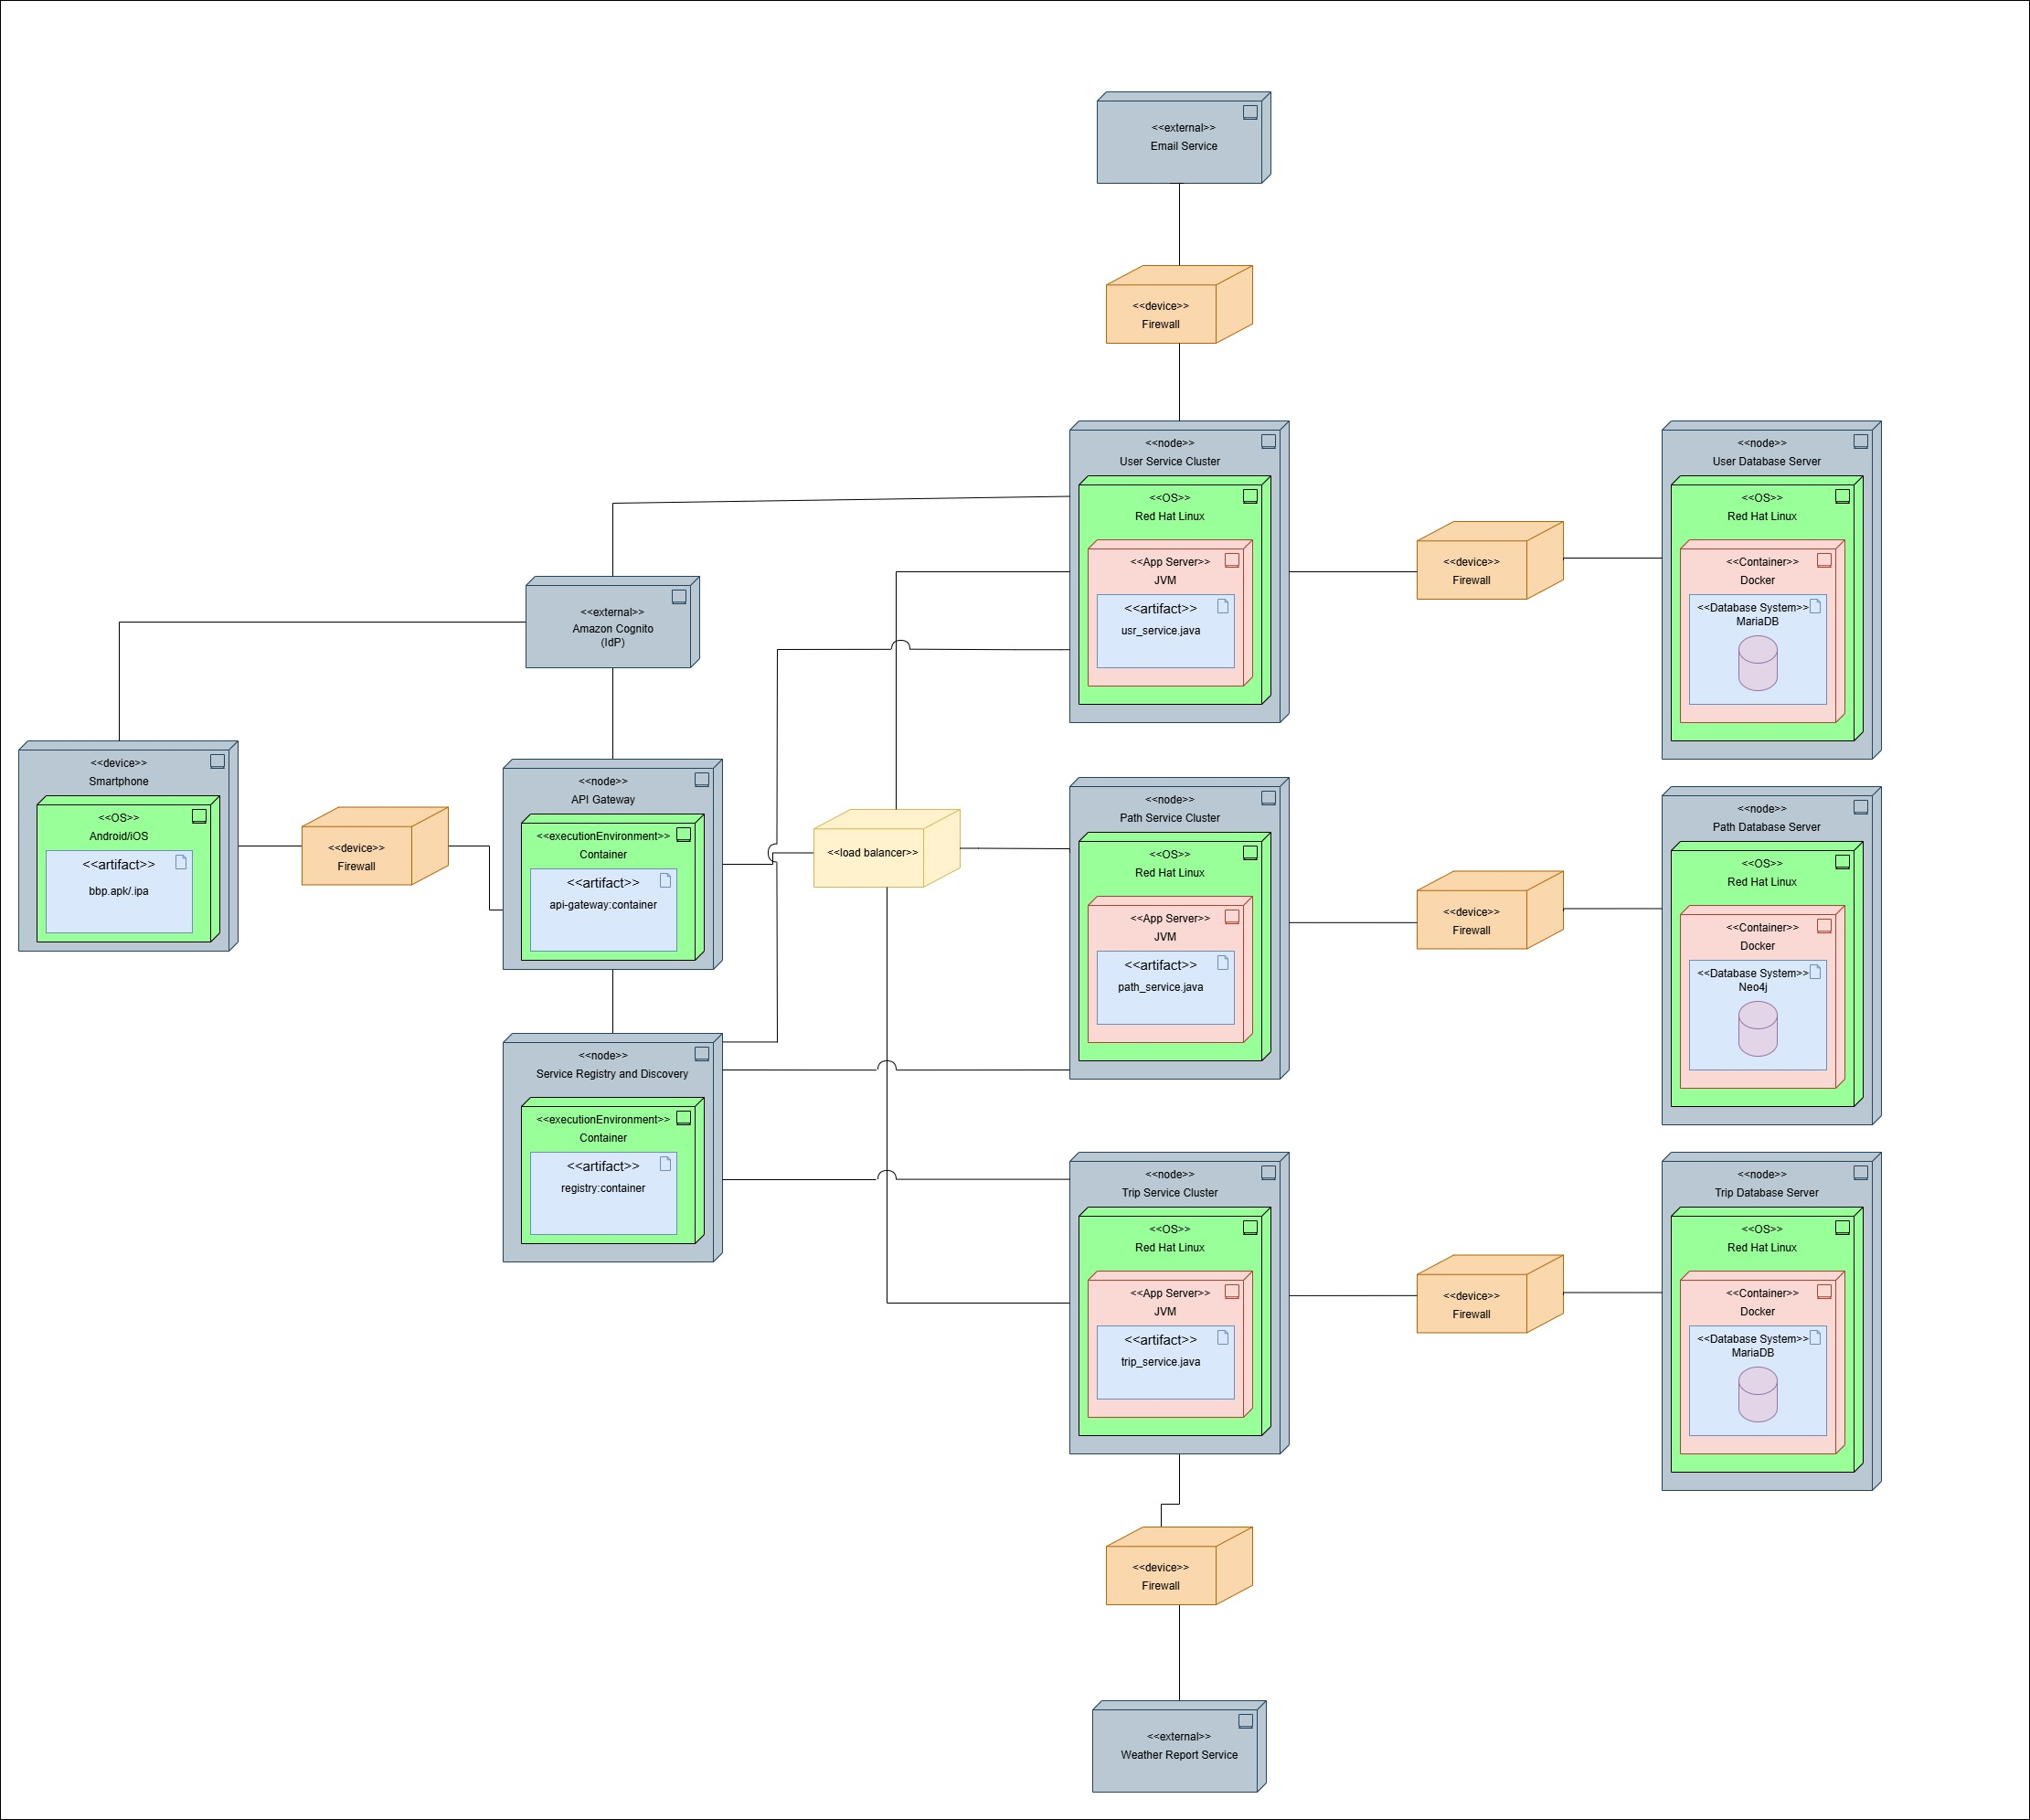
\includegraphics[width=0.91\textwidth]{DD/Images/Deployment Diagrams/Main-Deployment-Diagram.jpg}
\caption{\label{fig:componentDiagram} Deployment Diagram.}
\end{figure}

The diagram presents the relationships and the flow of data among the following components.

\begin{itemize}
    \item \textbf{Smartphone}: Hosts the Mobile BBP App, executing client-side presentation logic, GPS/sensor data capture, and map rendering via Google Maps SDK. Here the data is captured and sent to the backend services. 

    \item \textbf{API Gateway}: Single entry point for client requests, handling routing, authorization (via IdP), rate limiting, and service discovery integration.

    \item \textbf{Service Registry}: Centralized directory for dynamic service registration and discovery, enabling the API Gateway to locate available microservice instances. Also responsible for checking the health of instances via heartbeat. ~\cite{heartbeat}

    \item \textbf{User/Path/Trip Cluster}: Server orchestration groups hosting multiple instances of User, Path, and Trip Services for scalability and high availability.
    
    \item \textbf{User/Path/Trip Database}: Dedicated, per-service relational or NoSQL databases storing user profiles, path metadata/obstacles, and trip records/metrics respectively.
    
    \item \textbf{External Components}: Third-party services including Google Maps (geospatial), Email Delivery (notifications), and Weather API (trip enrichment), accessed via secure outbound connections.
\end{itemize}

\subsection{Component Interfaces}
The following diagram provides a comprehensive high level depiction of the interfaces and their associated methods offered by each component within the BBP platform. It is essential to acknowledge that the delineated methods do not precisely mirror the final version intended for implementation; rather, they serve as a logical representation

\begin{figure}[H]
\centering
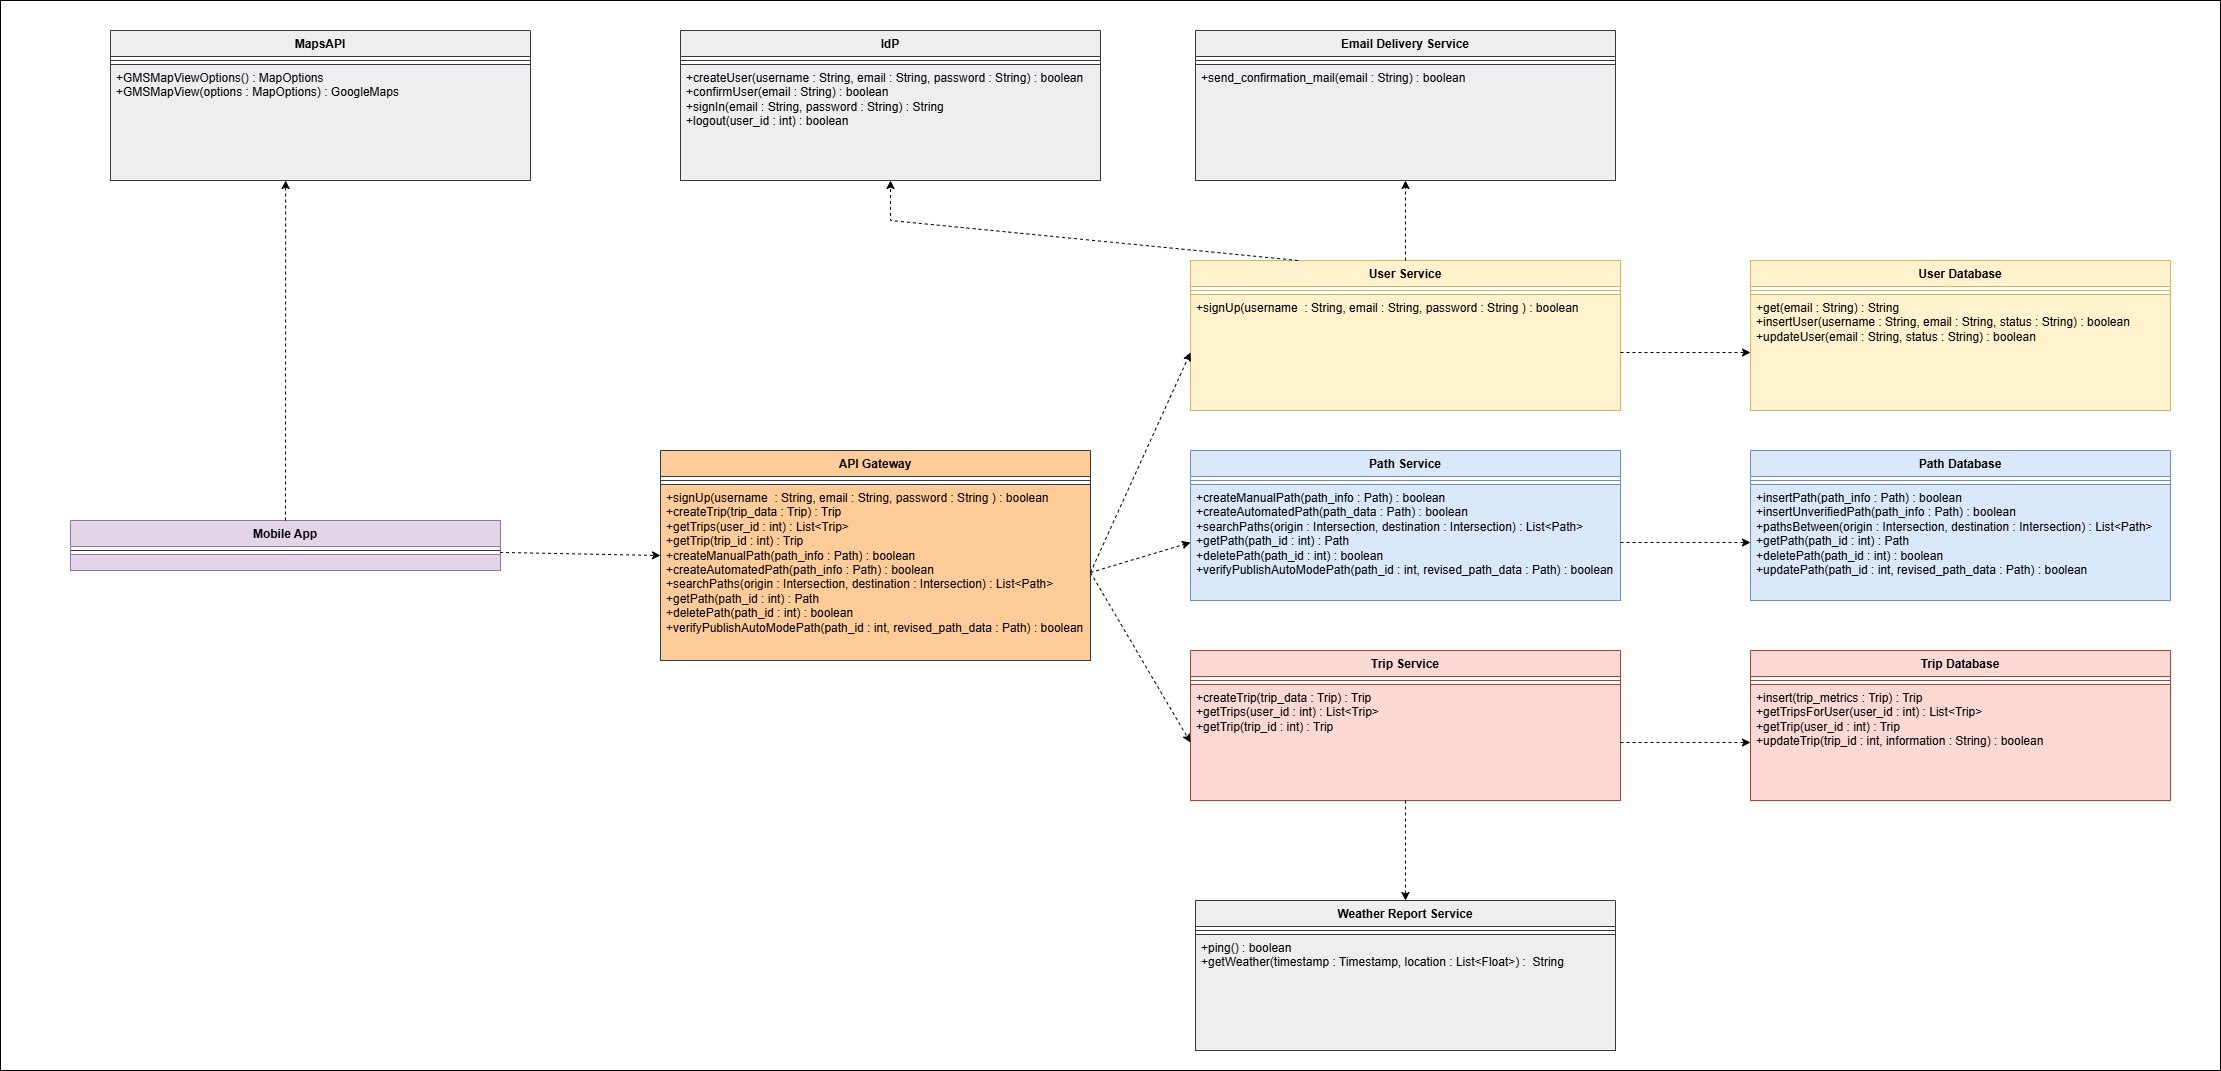
\includegraphics[width=\textwidth]{DD/Images/Component Diagrams/Interfaces.jpg}
\caption{\label{fig:runtimeDiagram} Interfaces diagram for BBP.}
\end{figure}


\pagebreak
\subsection{Runtime View}

This section presents several practical use cases of the system, illustrated by sequence diagrams.

\subsubsection*{Register}

\begin{figure}[H]
\centering
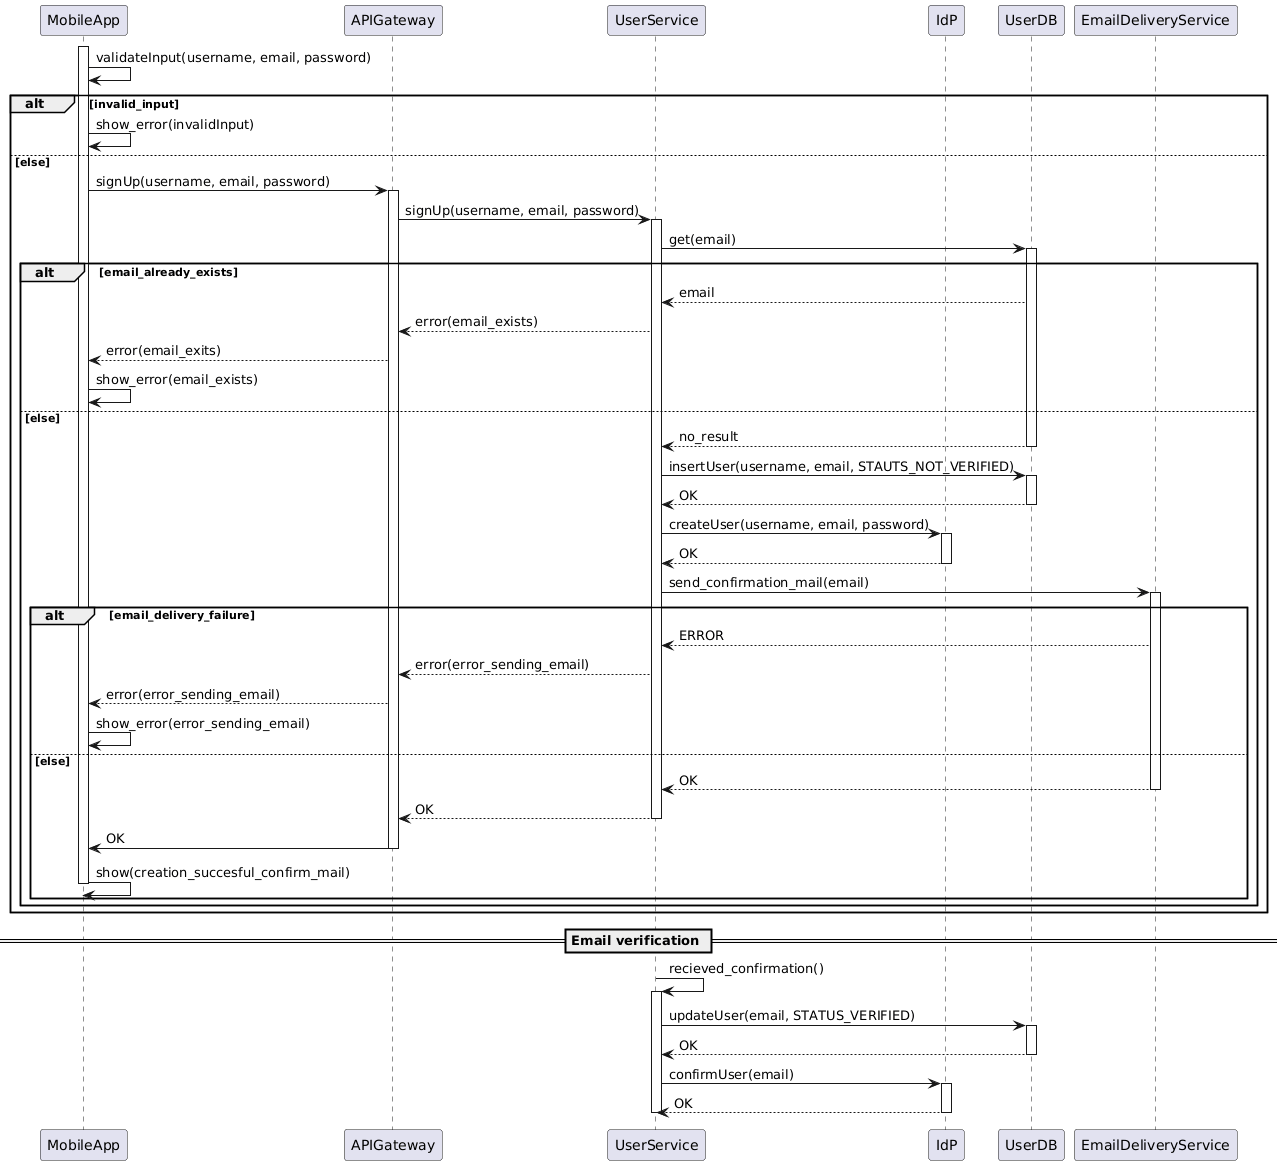
\includegraphics[width=\textwidth]{DD/Images/Runtime Diagrams/registerRuntime.png}
\caption{\label{fig:runtimeDiagram} Register runtime diagram.}
\end{figure}

The \textit{Sign-Up} phase shows the Mobile App submitting user details via API Gateway to User Service, which checks for email uniqueness in User DB. Then, it registers the user into the IdP and sends a confirmation account email. Once there is user confirmation for account completion the user service updates the user in the service database and IdP.

\pagebreak

\subsubsection*{Login}

\begin{figure}[H]
\centering
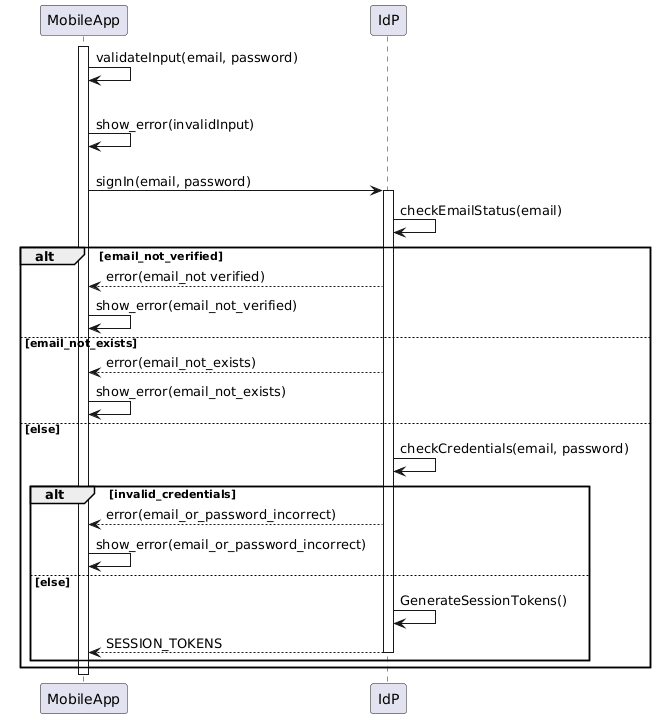
\includegraphics[width=\textwidth]{DD/Images/Runtime Diagrams/loginRuntime.png}
\caption{\label{fig:runtimeDiagram} Login runtime diagram.}
\end{figure}

The \textit{Login} phase shows the Mobile App submits credentials to the IdP, which first verifies user existence and account status, then authenticates the credentials. Upon success, session tokens are issued; otherwise, an appropriate error is returned.

\pagebreak

\subsubsection*{Search Paths}

\begin{figure}[H]
\centering
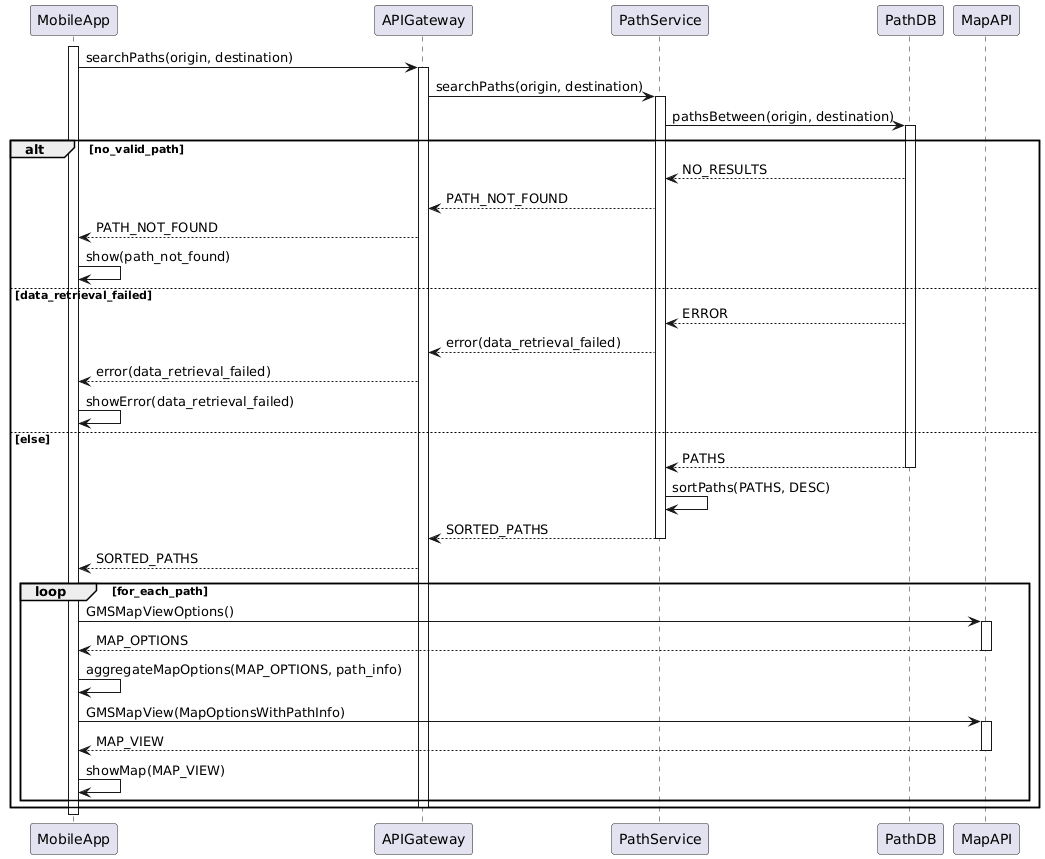
\includegraphics[width=\textwidth]{DD/Images/Runtime Diagrams/searchPathsRuntime.png}
\caption{\label{fig:runtimeDiagram} Search Paths runtime diagram.}
\end{figure}

The \textit{Search Path} phase shows the Mobile App sends origin and destination via API Gateway to Path Service, which queries Path DB for matching bike paths. Results may include zero, one, or multiple paths based on available data.

\pagebreak

\subsubsection*{Record Trip}

\begin{figure}[H]
\centering
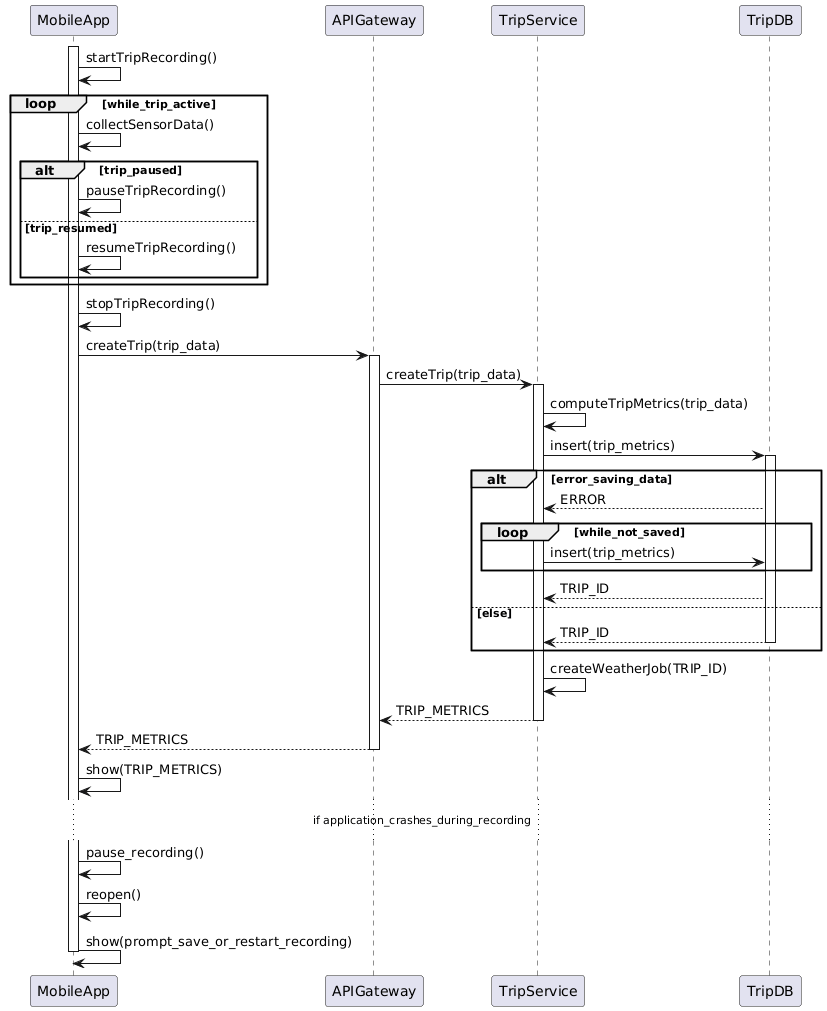
\includegraphics[width=\textwidth]{DD/Images/Runtime Diagrams/recordTripRuntime.png}
\caption{\label{fig:runtimeDiagram} Record Trip runtime diagram.}
\end{figure}

The \textit{Record Trip} phase shows the Mobile App gathers trip data from the device sensors. Data is then sent to Trip Service via API. Trip Service creates trip records in Trip DB, computes metrics, and schedules weather enrichment jobs.

\pagebreak

\subsubsection*{Attach Weather Information}

\begin{figure}[H]
\centering
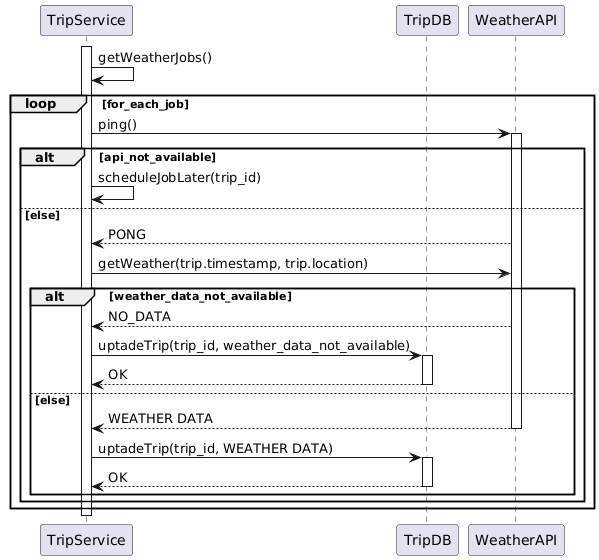
\includegraphics[width=\textwidth]{DD/Images/Runtime Diagrams/attachWeatherInfoRuntime.png}
\caption{\label{fig:runtimeDiagram} Attach weather information runtime diagram.}
\end{figure}

The \textit{Attach weather information} phase shows the Trip Service listing the scheduled weather jobs. For each it verifies the availability of the weather API, then making the request for weather information. It finally attaches the information to the corresponding trip in the service database.

\pagebreak

\subsubsection*{Review Trip}

\begin{figure}[H]
\centering
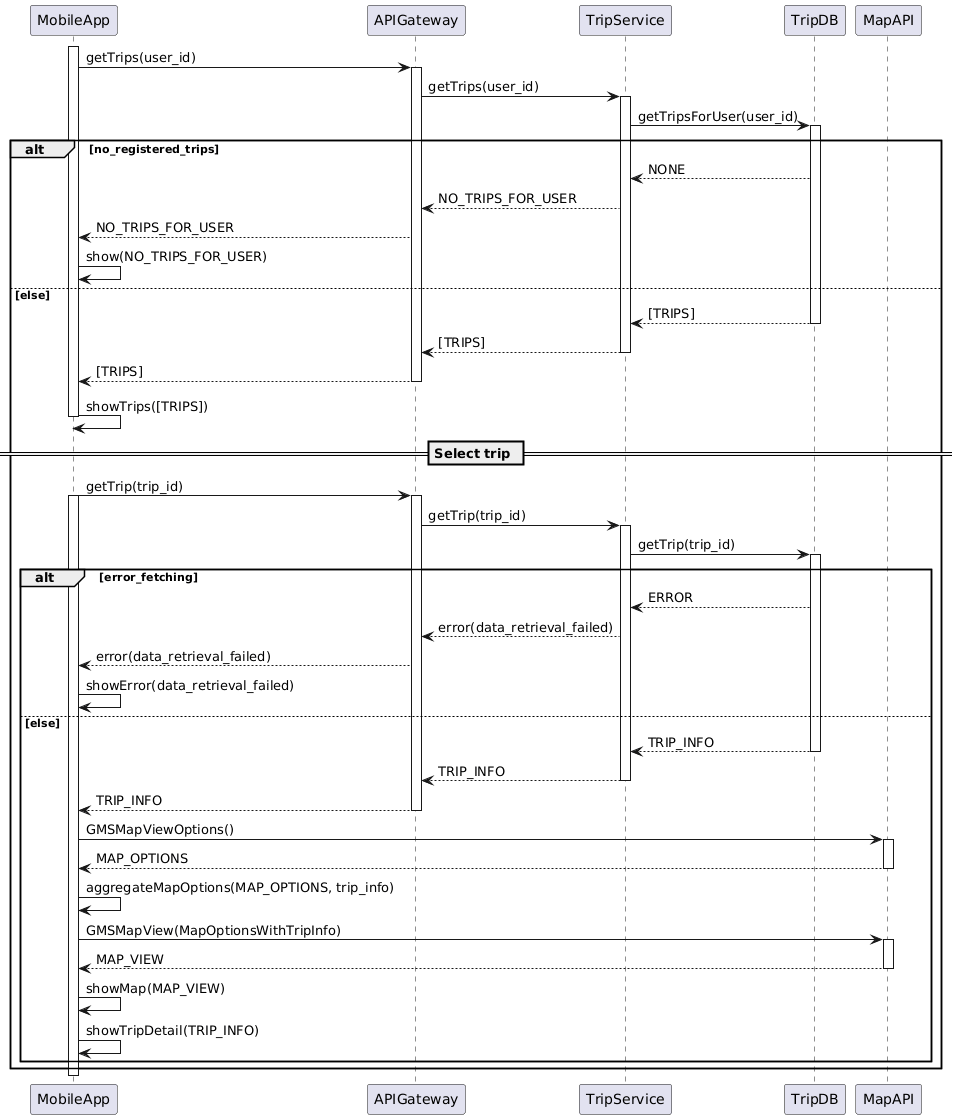
\includegraphics[width=\textwidth]{DD/Images/Runtime Diagrams/reviewTripRuntime.png}
\caption{\label{fig:runtimeDiagram} Review trip runtime diagram.}
\end{figure}

The \textit{Review Trip} phase shows Mobile App requesting the list of trips for a user to the Trip Service via API gateway. Either none are returned or a list of trips. Then one trip is selected and is requested from the mobile app, the service then returns the corresponding information and gets displayed.

\pagebreak

\subsubsection*{Enable Automated Mode}

\begin{figure}[H]
\centering
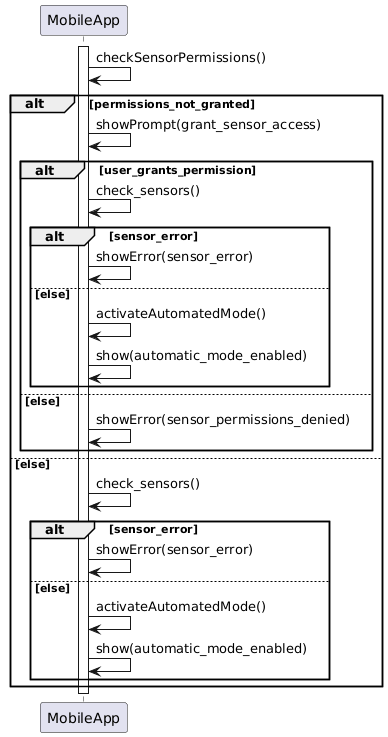
\includegraphics[scale=0.7]{DD/Images/Runtime Diagrams/enableAutoModeRuntime.png}
\caption{\label{fig:runtimeDiagram} Enable automated mode runtime diagram.}
\end{figure}

The \textit{Enable automated mode} phase shows Mobile App checking sensor permissions. If not granted, it prompts the user to grant access. If granted, the app checks sensors availability and starts gathering data in the background. 

\pagebreak

\subsubsection*{Disable Automated Mode}

\begin{figure}[H]
\centering
\includegraphics[scale=0.7]{DD/Images/Runtime Diagrams/disableAutoModeRuntime.png}
\caption{\label{fig:runtimeDiagram} Disable automated mode runtime diagram.}
\end{figure}

The \textit{Disable automated mode} phase shows Mobile App checking if a trip or path recording is in progress, if yes then it stops the recording. Then it stops gathering sensor data and stops background execution. 

\pagebreak

\subsubsection*{Create Manual Path}

\begin{figure}[H]
\centering
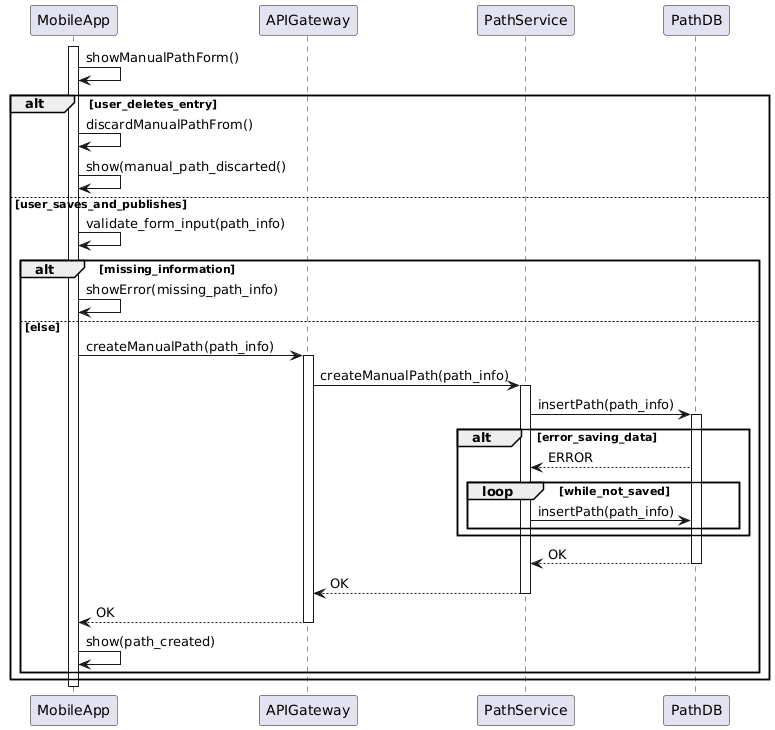
\includegraphics[width=\textwidth]{DD/Images/Runtime Diagrams/createManualPathRuntime.png}
\caption{\label{fig:runtimeDiagram} Create manual path runtime diagram.}
\end{figure}

The \textit{Create manual path} phase shows Mobile App showing the manual path form, then the user fill in the information. The user can decide whether discard the form or publish the path. If the decision is to publish the Mobile App validates the form information and sends it to the Path service via API gateway. The Path service saves this information in the service database.

\pagebreak

\subsubsection*{Record Path with Automated Mode}

\begin{figure}[H]
\centering
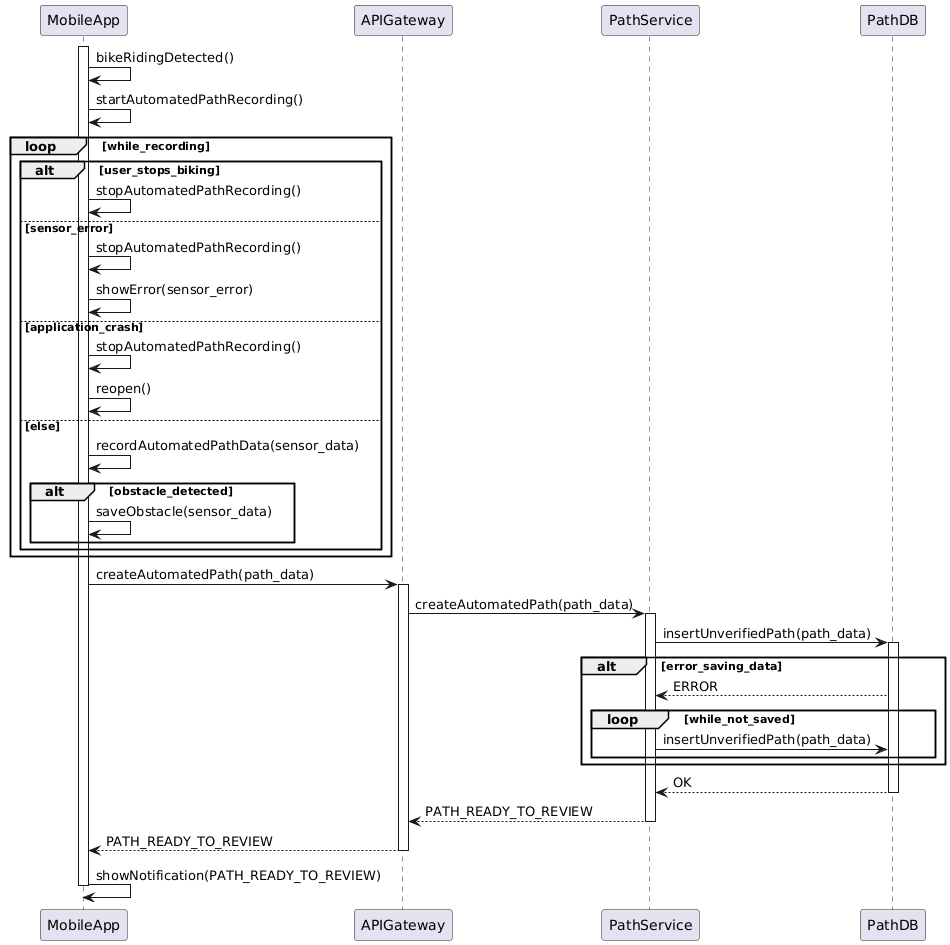
\includegraphics[width=\textwidth]{DD/Images/Runtime Diagrams/recordPathAutoMode.png}
\caption{\label{fig:runtimeDiagram} Record path with automated mode runtime diagram.}
\end{figure}

The \textit{Record path with automated mode} phase shows Mobile App detecting a bike ride and start a path recording. While the user rides the bike the Mobile app records data from the sensors and detects obstacles. It stops the recording if the user stops riding, a sensor error occurs or the application crashes. It then sends the collected data to the Path service via API gateway. The services storage this data on the service data base and marks it as unverified for later user revision.

\pagebreak

\subsubsection*{Publish Pre-recorded Path in Automated Mode}

\begin{figure}[H]
\centering
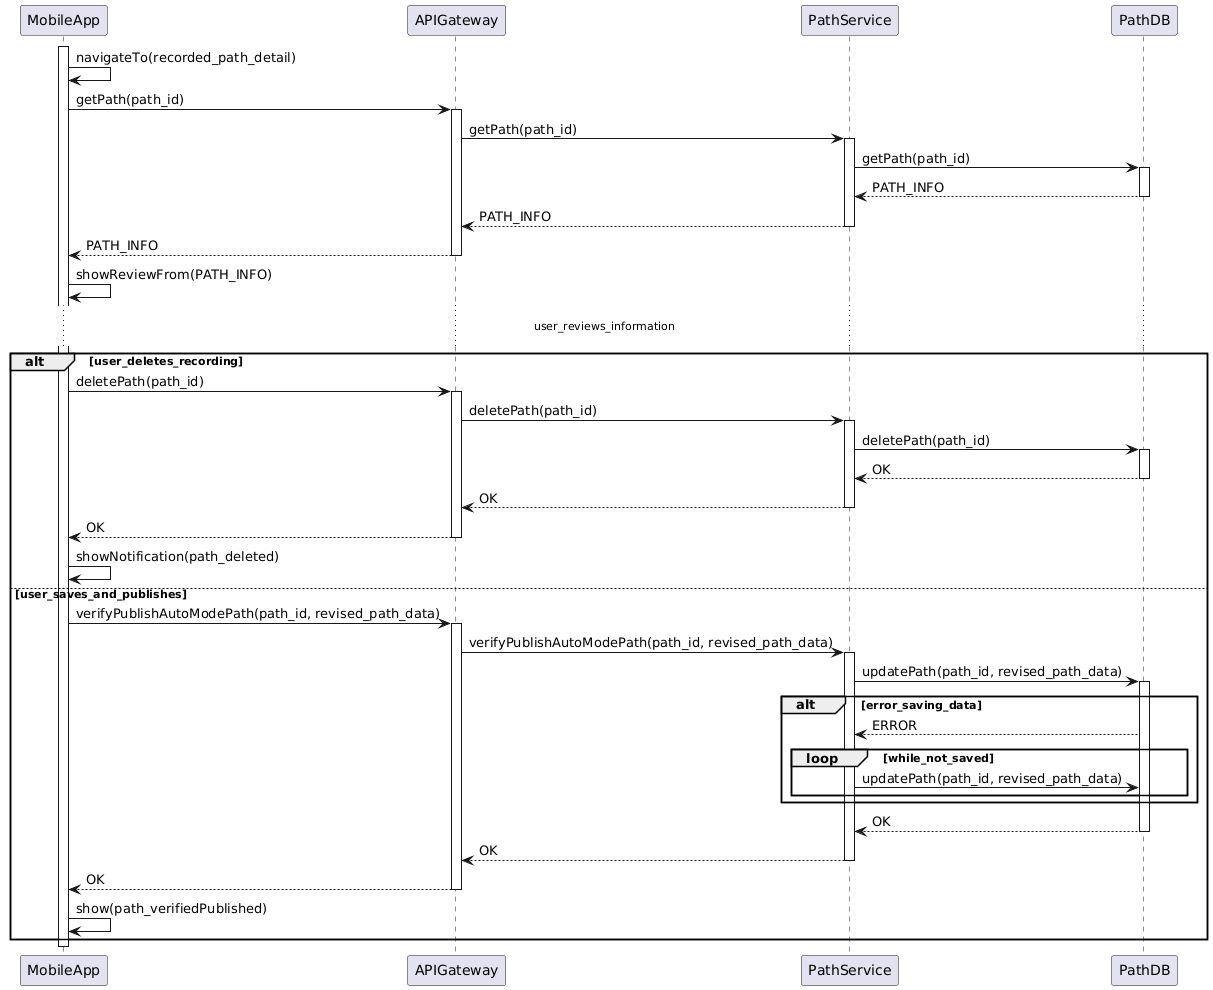
\includegraphics[width=\textwidth]{DD/Images/Runtime Diagrams/publishAutoModePathRuntime.png}
\caption{\label{fig:runtimeDiagram} Publish pre-recorded path in automated mode runtime diagram.}
\end{figure}

The \textit{Publish pre-recorded path in automated mode} phase shows Mobile App navigating to the detail of path pending review. Then the user reviews and can decide whether to discard it or publish it. In case of discard, the mobile app sends a deletion request to the path service and the path gets eliminated from the service database. Otherwise the mobile app sends a request to the path service to update the path with the revised information.

\pagebreak

\subsubsection*{Logout}

\begin{figure}[H]
\centering
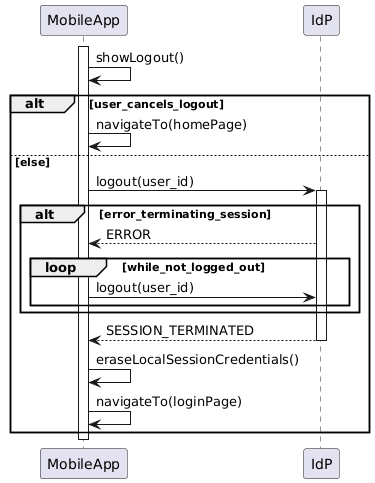
\includegraphics[scale=0.7]{DD/Images/Runtime Diagrams/logoutRuntime.png}
\caption{\label{fig:runtimeDiagram} Logout runtime diagram.}
\end{figure}

The \textit{Logout} phase shows Mobile App showing the user the logout dialog. The user can either cancel or confirm the logout action. In case of confirmation, the mobile app erases local cache, requests the IdP to terminate session credentials and navigates to the login page.


\pagebreak
\subsection{Selected Architectural Styles and Patterns}
%Ale is doing this
Here below are discussed the utilized architectural styles and patterns:
\begin{itemize}
    \item \textbf{Microservices architecture}: the chosen system architecture is a microservices architecture, being the natural approach for this type of application. In this case, as a matter of fact, the single main features (User, Trip and Path management) are easily distinguishable and with a very separated runtime, making the microservices architecture the best choice. In this approach, every feature is run by a different component (or set of components) specialized for a single task. The application logic is deliberately decoupled from the data tier to ensure a clear separation of concerns and to promote specialization.. \newline
            \textbf{Main advantages}:
            \begin{itemize}[label = -]
                \item Improved resilience
                \item Fine-grained scaling
                \item Easier deployment
                \item Technology-neutral protocols (REST APIs, used for communication by all of the microservices)
                \item Concurrency
            \end{itemize}

    \item \textbf{Security pattern: API Gateway \cite{apigateway}}: in a microservice architecture, an API Gateway is essential. It is a centralized entry point that manages and routes requests from clients to the correct microservice. Introducing caching at this level may help latency.
    \newline
    \textbf{Main advantages}:
            \begin{itemize}[label = -]
                \item Single gateway for clients
                \item Routing and Load balancing
                \item Authentication and Authorization methods
            \end{itemize}
    The main challenges to consider are:
    \begin{itemize}[label = -]
                \item Possible performance bottleneck and single point of failure: to make sure they can support the load, different instances of the gateway are necessary, with also adding load balancing if needed;
                \item Scalability: consider horizontal scalability and load balancing
                \item Security risks (if not configured correctly)
            \end{itemize}
            
    \item \textbf{Routing pattern: Service Registry and Discovery \cite{registry}}: to guarantee service discovery and reachability, a service registry and discovery layer is a must have in this architecture. The API Gateway looks up for available services using the nodes in this layer. The single service instances will register to this layer, and notify them of their availability using a heartbeat signal.\newline
    \textbf{Main advantages}:
            \begin{itemize}[label = -]
                \item More efficient load balancing
                \item Fault tolerance (service discovery can route traffic to other healthy instances)
                \item Dynamic environment, without manual intervention
                \item Easier scalability
            \end{itemize}

\end{itemize}
\subsection{Other Design Decisions}
\begin{itemize} 

    \item \textbf{Security: Amazon Cognito (IdP) \cite{cognito}}: to guarantee a better authentication mechanism, Amazon Cognito is a great choice. It can be used to create "pools" of users with a predetermined set of permissions, that acquire a specific authorization token (JWT) to pass to the API Gateway. In this way, it is possible to identify the groups of users and their permissions.
    
    \item \textbf{GDBMS}: using a Graph Database Management System seemed to suit better the information stored in the path database. In fact, it is easier to perform queries, if data is structured as nodes (intersections) and edges (roads), thanks to the better overlap between reality and model.

\end{itemize}



